\documentclass[12pt,4paper]{article}

\usepackage{tabularx}

\usepackage{minted}
\usepackage{textcomp}
\usepackage[scaled]{beramono}
\usepackage{stmaryrd}        % [|a, b|]
\usepackage[T1]{fontenc}
\usepackage[utf8]{inputenc}  % Accents codés dans la fonte

\usepackage{amsmath}         % Maths de base
\usepackage{amssymb}

\usepackage[svgnames]{xcolor}% Pour PythonTeX
\usepackage[top=1cm, bottom=2cm, left=1cm, right=1cm]{geometry}

\usepackage[linesnumbered,ruled,vlined]{algorithm2e}

%%% Coloring the comment as blue
\newcommand\mycommfont[1]{\footnotesize\ttfamily\textcolor{blue}{#1}}
\SetCommentSty{mycommfont}

\usepackage{subcaption}	     % Sous figures

\usepackage{tgpagella}       % Fontes
\usepackage{tgadventor}
\usepackage{inconsolata}

\usepackage{enumitem}	     % Personalisation des puces des listes
\usepackage{pifont}

\usepackage{pythontex}       % PythonTeX

\usepackage{graphicx}        % Inclusions de figures

\usepackage{tikz}
\usepackage[framemethod=TikZ]{mdframed}

% Environnement de présentation code Python
\newenvironment{code}{%
\begin{mdframed}[linecolor=Green,innerrightmargin=30pt,innerleftmargin=30pt,
backgroundcolor=Black!5,
skipabove=10pt,skipbelow=10pt,roundcorner=5pt,
splitbottomskip=6pt,splittopskip=12pt]
}{%
\end{mdframed}
}

% Puces
\setenumerate[1]{label=\arabic*.}
\setenumerate[2]{label=(\alph*)}

\setitemize[1]{label=\ding{56}}
\setitemize[2]{label=\textbullet}
\setitemize[3]{label=o}
\setitemize[4]{label=$\square$}
\setitemize[5]{label=-}

\title{Solution TD 1 : Introduction to algorithms and data structures}
\author{\textsc{Doriath Döhler} Gabriel}

\begin{document}
\maketitle
\begin{enumerate}

% 1.
\item $\mathcal{O}$, $\Omega$ and $\Theta$ notations\\
Prove or disprove :
\begin{enumerate}

% 1. (a)
\item $f(n) + g(n) = \Theta(\min(f(n), g(n)))$\\
False : let $\forall n \in \mathbb{N}, f(n) = n$ and $g(n) = n^2$.\\
$f(n) + g(n) \in \Theta(n^2) \neq \Theta(n) = \Theta(\min(f(n), g(n))) = n$\\
$\forall n \in \mathbb{N}, f(n) = (-1)^n$ and $g(n) = (-1)^{n+1}$ also constitue a conterexample but
negative complexity are rare...

% 1. (b)
\item $g(n) - h(n) = \Theta(f(n))$, where $g(n), f(n) \in \Theta(f(n))$\\
False : let $\forall n \in \mathbb{N}, f(n)=g(n)=h(n)$\\
We have $g(n), h(n) \in \Theta(f(n))$ but $g(n) - f(n) = 0 \notin\Theta(n) = \Theta(f(n))$

% 1. (c)
\item $\Theta(f(n)) + \Omega(f(n)) = \mathcal{O}(f(n))$\\
False : let $\forall n \in \mathbb{N}, f(n) = n$.\\
$n = \Theta(f(n))$ and $e^n = \Omega(f(n))$ but $n + e^n \notin \mathcal{O}(n)$

\end{enumerate}


% 2.
\item Classic assymptotic relations\\
Show that $n!=o(n^n)$ and $\log(n!)=\Theta(n\log(n))$.

\begin{itemize}
\item Proof with Stirling.\\
Reminder : $n! \sim \sqrt{2\pi n} \left(\frac{n}{e}\right)^n$.
$n!=o(n^n)$ follows. By composing with an equivalent we get :
$\log(n!)=\Theta(n\log(n))$. Note that we can apply $\log$ on the Stirling
formula because $n! \to \infty$.

\item Elementary proof.\\
$0 \leq \frac{n!}{n^n} = \frac{n \times (n - 1) \dots \times 1}{n \times \dots \times
n} = \prod_{k=1}^n \frac{k}{n} \leq \frac{1}{n} \to 0$ so $n! = o(n^n)$.\\
$\log(n!)=\sum_{k=1}^n\log(k)\geq \sum_{n\geq k\geq\frac{n}{2}}
\log(k) \in \Theta(n\log(n))$\\
We conclude with : $\log(n!) = \sum_{k=1}^n \log(k) \leq \sum_{k=1}^n \log(n) = n \log(n)$

\item Jérôme's elegant proof.\\
By concavity of the logarithm we have : $\forall n \in \mathbb{N}^*, \forall
1 \leq k \leq
n, \log(k) \geq \frac{\log(n)}{n-1}(k - 1)$.\\
For example with $n=100$ :\\

\begin{center}
\includegraphics[width=\linewidth]{/home/gab/Documents/ens/info/algorithmique/td/1/jerome.png}
\end{center}

Hence : $\log(n!)=\sum_{k=2}^n\log(k)\geq \sum_{k=2}^n
\frac{\log(n)}{n-1}(k-1) \geq \frac{\log(n)}{n}\sum_{k=2}^n (k - 1) \in
\Theta(n\log(n))$\\
We conclude with : $\log(n!) = \sum_{k=1}^n \log(k) \leq \sum_{k=1}^n \log(n) = n \log(n)$

\end{itemize}

% 3.
\item Prove that : $\forall a \in \mathbb{R}, \forall b \in \mathbb{R}^*_+,
(n + a)^b = \Theta(n^b)$\\
If $a \geq 0$ then
$\forall n \in \mathbb{N}^*, 0 \leq \frac{n^b}{(n + a)^b} \leq 1$ so $n^b = \mathcal{O}((n + a)^b)$. We
also have $\forall n \in \mathbb{N}^*, \frac{(n + a)^b}{n^b} = (1 +
\frac{a}{n})^b \leq (1 + a)^b$ so $(n + a)^b \in \mathcal{O}(n^b)$. Finally we
have that $(n + a)^b \in \Theta(n^b)$.\\
If $a < 0$ a similar method proves the result (left as an exercice to the
reader).\\

% 4.
\item Two stack in one array.

\begin{algorithm}[H]
\DontPrintSemicolon

\SetKwFunction{Fcreate}{create}
\SetKwFunction{FpopOne}{pop1}
\SetKwFunction{FpopTwo}{pop2}
\SetKwFunction{FpushOne}{push1}
\SetKwFunction{FpushTwo}{push2}

\SetKwProg{Fn}{Function}{:}{}
\Fn{\Fcreate{n}}{
    a = Array.make(n, 0)\;
    i = 0\;
    j = n - 1\;
    \KwRet a, i, j\;
}
\;

\SetKwProg{Fn}{Function}{:}{}
\Fn{\FpopOne{a, i, j}}{
    \If {i > 0} {
        i = i - 1\;
        \KwRet a[i]
    } \Else {
        raise Stack1Empty
    }
  }
\;

\SetKwProg{Fn}{Function}{:}{}
\Fn{\FpopTwo{a, i, j}}{
    \If {j < n - 1} {
        i = j + 1\;
        \KwRet a[j]
    } \Else {
        raise Stack2Empty
    }
  }
\;

\SetKwProg{Fn}{Function}{:}{}
\Fn{\FpushOne{a, i, j, x}}{
    \If {i = j + 1} {
        raise Stack1Full
    } \Else {
        a[i] = x\;
        i = i + 1
    }
  }
\;

\SetKwProg{Fn}{Function}{:}{}
\Fn{\FpushTwo{a, i, j, x}}{
    \If {i = j + 1} {
        raise Stack2Full
    } \Else {
        a[j] = x\;
        j = j - 1
    }
  }
\;

\end{algorithm}

$pop1$, $pop2$, $push1$ and $push2$ clearly take $\mathcal{O}(1)$ time. Here is
an implementation in python :

\begin{code}
\begin{pyblock}[][numbers=left]
class Double_stack:
    def __init__(self, n):
        self.n = n
        self.a = [None] * n
        self.i = 0
        self.j = n - 1

    def __str__(self):
        return f'n : {self.n}, i : {self.i}, j : {self.j}, a : {self.a}'

    def __repr__(self):
        return str(self)

    @property
    def is_not_full(self):
        return self.i != self.j + 1

    def pop1(self):
        assert self.i > 0, 'stack1empty'
        self.i -= 1
        return self.a[self.i]

    def pop2(self):
        assert self.j < self.n - 1, 'stack2empty'
        self.j += 1
        return self.a[self.j]

    def push1(self, x):
        assert self.is_not_full, 'stack1full'
        self.a[self.i] = x
        self.i += 1

    def push2(self, x):
        assert self.is_not_full, 'stack2full'
        self.a[self.j] = x
        self.j -= 1
\end{pyblock}
\end{code}
Note that we could use a similar strategy to exercice 8 in order to deal with
overflow.

% 5.
\newpage
% 5. (a)
\item Implementation of a stack with two queues.\\
\begin{enumerate}

\item With two queues :\\
\begin{algorithm}[H]
\DontPrintSemicolon

\SetKwFunction{Fcreate}{create}
\SetKwFunction{Fpush}{push}
\SetKwFunction{Fpop}{pop}

\SetKwProg{Fn}{Function}{:}{}
\Fn{\Fcreate{}}{
    $Q_1$ = createEmptyQueue()\;
    $Q_2$ = createEmptyQueue()\;
    $sizeQ_1$ = 0\;
    \KwRet $Q_1$, $Q_2$, $sizeQ_1$\;
}
\;

\SetKwProg{Fn}{Function}{:}{}
\Fn{\Fpush{$Q_1$, $Q_2$, $sizeQ_1$, $x$}}{
        pushQueue($Q_1$, $x$)\;
}
\;

\SetKwProg{Fn}{Function}{:}{}
\Fn{\Fpop{$Q_1$, $Q_2$, $sizeQ_1$}}{
    \If {$sizeQ_1$ = 0} {
        raise EmptyStack
    }
    $initialSizeQ_1$ = $sizeQ_1$\;
    \While {$sizeQ_1$ > 1} {
        x = popQueue($Q_1$)\;
        pushQueue($Q_2$, x)\;
        $sizeQ_1$ = $sizeQ_1$ - 1\;
    }\;
    x = popQueue($Q_1$)\;
    $sizeQ_1$ = $sizeQ_1$- 1\;
    $Q_1$, $Q_2$ = $Q_2$, $Q_1$\;
    $sizeQ_1$ = $initialSizeQ_1$ - 1\;
    \KwRet x
  }
\;
\end{algorithm}

\newpage
% 5. (b)
\item With only one queue :\\
\begin{algorithm}[H]
\DontPrintSemicolon

\SetKwFunction{Fcreate}{create}
\SetKwFunction{Fpush}{push}
\SetKwFunction{Fpop}{pop}

\SetKwProg{Fn}{Function}{:}{}
\Fn{\Fcreate{}}{
    $Q$ = createEmptyQueue()\;
\    \KwRet $Q$\;
}
\;

\SetKwProg{Fn}{Function}{:}{}
\Fn{\Fpush{$Q$, $x$}}{
        pushQueue($Q$, $x$)\;
}
\;

\SetKwProg{Fn}{Function}{:}{}
\Fn{\Fpop{$Q$}}{
    \If {isEmptyQueue($Q$)} {
        raise EmptyStack
    }
    push($Q$, "end")\;
    x = popQueue($Q$)\;
    last = Null\;
    \While {x $\neq$ "end"} {
        \If {last $\neq$ Null} {
            push($Q$, last)
        }
        last = x\;
        x = popQueue($Q$)
    }\;
    \KwRet last
  }
\;
\end{algorithm}
Complexity : push and create are $\Theta(1)$ but pop is $\Theta(n)$. Maybe there is a better way to do it ?
\end{enumerate}

% 6.
\item Palindrome detection.
\begin{enumerate}
% 6. (a)
\item Solution in Ocaml :\\
\begin{code}
\begin{minted}{ocaml}
let rec rev ?(acc=[]) = function
    | []     -> acc
    | t :: q -> rev ~acc:(t :: acc) q

let rec equal l1 l2 = match l1, l2 with
    | [], []             -> true
    | [], _ | _, []      -> false
    | t1 :: q1, t2 :: q2 -> t1 = t2 && equal q1 q2

let isPalindrome l = egal l (rev l)
\end{minted}
\end{code}

\newpage
% 6. (b)
\item Solution in Ocaml (we assume that the garbage collector does its jobs) :\\
\begin{code}
\begin{minted}{ocaml}
let rec split ?(l1=[]) l k =
    if k = 0 then
        l1, l
    else (
        match l with
            | []     -> failwith "error ;)"
            | t :: q -> split ~l1:(t :: l1) q (k - 1)
    )

let isPalindrome l =
    let n = List.length l in
    n mod 2 = 0 && (
        let l1, l2 = split l (n / 2) in
        egal l1 (rev l2)
    )
\end{minted}
\end{code}
Note that all recursive function here are tail recursive so no space for a stack is requiered.

\end{enumerate}
% 7
\item Implementation of a queue using two stacks.
\begin{itemize}
\item $create\_empty$ : create two stacks $S_1$ and $S_2$.
\item $push$ $x$ : add $x$ to $S_1$.
\item $pop$ : if $S_2$ is not empty then pop from $S_2$ else transfert (one by
one) all the
elements of $S_1$ into $S_2$. If $S_2$ is still empty then the queue is empty else pop from $S_2$.
\end{itemize}
Implementation is left as an exercice.\\
Analysis : During $n$ operations on the data structure, there are at most $n$
elements going on the queue. Each element is at most added to $S_1$ then
transfered from $S_1$ to $S_2$ and then popped from $S_2$. These three
operations take constant time. As a consequence, doing $n$ operations on the data
struture takes $\Theta(n)$ time. Hence the $\Theta(1)$ amortized time
complexity.
In other words, if you need to tranfert the $k$ elements of $S_1$ to $S_2$
(wich takes $\Theta(k)$ time), you
have already done $\Theta(k)$ operations to fill $S_1$. Note that queues can
also be implemented with dynamic circular arrays (tableau dynamique circulant en
français) or doubly linked lists.


% 8.
\item Dynamic arrays. (Similar to python's lists.)

\begin{enumerate}

% 8. (a)
\item

\begin{itemize}
\item $create\_empty$ : create an array $a$ of length 2. Set $n \leftarrow 2$.
\item $access$ $i$ : if $i < n$ then return $a[i]$.
\item $set$ $i$ $x$ : if $i < n$ then $a[i] \leftarrow x$.
\item $insert$ $x$ : create an
array $b$ of length $2 n$, $b[0:n] \leftarrow a$, $b[n] \leftarrow x$, $a
\leftarrow b$ and $n
\leftarrow 2n$. (The garbage collector will destroy $b$).
\end{itemize}

Analysis : $access$, $set$ and $create\_empty$ all take $\Theta(1)$ time. Space is always bounded by
$3n+3$. Insertion takes $\Theta(n)$ time but we only have to use it when $a$ is
full. And in order for $a$ to be full we need to call $set$ $\frac{n}{2}$ times wich
takes $\Theta(n)$ time. All together, this gives an $\Theta(1)$ amortized
runing time.

% 8. (b)
\item Why would we want to reduce the size of $a$ ? After all, if $a$ is at
some point of size $n$ and later of size $k < n$ the space complexity will
still be
$n$. So why bother ? Lets describe an algorithm that uses $n$ dynamic
arrays :\\

\begin{algorithm}[H]
\DontPrintSemicolon
create $n$ dynamic arrays $a_1, \dots, a_n$\;
\For {$j \in \llbracket 1, n \rrbracket$} {
    \For {$k \in \llbracket 1, n \rrbracket$} {
        store k in $a_j$\;
    }
    \For {$k \in \llbracket 1, n \rrbracket$} {
        remove k from $a_j$\;
    }
}
\;
\end{algorithm}

Without reducing the size of the arrays when deleting elements the space
complexity is $\Theta(n^2)$ whereas when reducing the size of the arrays, the
space complexity is $\Theta(n)$.
This is much better.\\\\
First strategy : keep in memory the number of elements stored in $a$ (lets called that
$i$). When $2i<n$ resize the array by cutting its size by 2.\\
Analysis : This sadly doesn't work. Indeed, if we have $n$ elements stored in
$a$ of size $2n$, adding and then removing an element $n$ times will take
$\Theta(n^2)$ time for $\Theta(n)$ operations in total (including the insertion of
the first $n$ elements of $a$).

% 8. (c)
\item Second strategy : quadruple the size of $a$ when it is more than
$\frac{3}{4}$ full and cut the array size in 4 when it is less than
$\frac{1}{4}$ full. It can easily be proven (using the same techniques as
before) that this strategy gives a
$\Theta(1)$ amortized runing time for all operations.
\end{enumerate}

% 9.
\item Longest common subsequence.

\begin{enumerate}

% 9. (a)
\item Clearly, a greedy algorithm doesn't work here so lets use dynamic
programming. First of all lets define the subproblems :\\
$\forall i \in \llbracket 0, m \rrbracket, \forall j \in
\llbracket 0, n \rrbracket, P_{x, y}[i, j] := |LCS((x_1, \dots, x_i), (y_1,
\dots, y_j))|$.\\
For negative $i$ or $j$, $P_{x, y}[i, j] := 0$\\
We then find a relation between subproblems :
\begin{itemize}
\item
$
P_{x, y}[0, \_] = P_{x, y}[\_, 0] = 0
$
\item
$
\forall i \in \llbracket 0, m \llbracket,
\forall j \in \llbracket 0, n \llbracket,
P_{x, y}[i + 1, j + 1] =
\left\{ \begin{array}{ll}
		P_{x, y}[i, j] + 1 & \mbox{if } x_{i + 1} = y_{j + 1}\\
		\max(P_{x, y}[i + 1, j], P_{x, y}[i, j  + 1]) & \mbox{otherwise}

	\end{array}
\right.
$
\end{itemize}
Indeed : if $x_{i + 1} = y_{j + 1}$ we can just add $x_{i + 1}$ and $y_{j + 1}$ to $LCS((x_1, \dots, x_i), (y_1, \dots, y_j))$ to get a common subsequence of $(x_1, \dots, x_{i + 1})$ and $(y_1, \dots, y_{j + 1})$ of size $P_{x, y}[i, j] + 1$. This is optimal by optimality of $LCS((x_1, \dots, x_i), (y_1, \dots, y_j))$. If $x_{i + 1} \neq y_{j + 1}$ then either $x_i$ or $y_j$ is not in a longest common subsequence of $(x_1, \dots, x_i)$ and $(y_1, \dots, y_j)$. This proves $(*)$.\\
Finally we need to find an order to fill the table $P_{x, y}$. For example
columns by columns or row by row or diagonal by diagonal. Here any one of these
will work.

\begin{center}
\includegraphics[scale=0.1]{/home/gab/Documents/ens/info/algorithmique/td/1/base.png}
\includegraphics[scale=0.08]{/home/gab/Documents/ens/info/algorithmique/td/1/col.png}
\includegraphics[scale=0.08]{/home/gab/Documents/ens/info/algorithmique/td/1/row.png}
\includegraphics[scale=0.08]{/home/gab/Documents/ens/info/algorithmique/td/1/diag.png}
\includegraphics[scale=0.08]{/home/gab/Documents/ens/info/algorithmique/td/1/square.png}
\end{center}

Implementation in Ocaml :\\
\begin{code}
\begin{minted}{ocaml}
let lcs x y =
    let m = String.length x in
    let n = String.length y in
    let a = Array.make_matrix m n 0 in
    let p i j =
        if i >= 0 && j >= 0 then
            a.(i).(j)
        else
            0
    in

    for i = 0 to m - 1 do
        for j = 0 to n - 1 do
            a.(i).(j) <-
                if x.[i] = y.[j] then
                    p (i - 1) (j - 1) + 1
                else
                    max (p i (j - 1)) (p (i - 1) j)
        done;
    done;
    p (m - 1) (n - 1)
\end{minted}
\end{code}

Analysis : filling a case of the table takes $\Theta(1)$ time so the complexity
is $\Theta(nm)$ time and space.

% 9. (b)
\item For each $i$, $j$ we will store in $
P'_{x, y}[i, j] \leftarrow
\left\{ \begin{array}{ll}
		(i - 1, j - 1) & \mbox{if } x_i = y_j\\
		(i, j - 1) & \mbox{if } P_{x, y}[i, j - 1] > P_{x, y}[i - 1, j]
\mbox{and } x_i \neq y_j\\
		(i - 1, j) & \mbox{otherwise}
	\end{array}
\right.
$ thus remembering the choices we make while constructing $P_{x, y}$.
\\
From that we can recover the longest common subsequence. Note that the
asymptotic time and space complexity doesn't change.

% 9. (c)
\item Remark :\\One row/column/diagonal only depends on the one/one/two previous
row/column/diagonals. Therefore we only need to store the last row or the last
column or the last two diagonals. This technique gives a $\Theta(\min(m, n))$
space complexity (not acounting for the space to store $x$ and $y$. Sadly this
only works if want the length of the $LCS$ and not one actual $LCS$.
\end{enumerate}

% 10.
\item Interval graphs.

\begin{enumerate}
    % 10. (a)
    \item Greedy strategy : choose the task that finish the soonest.\\
    Analysis : sorting the tasks by finish time takes $\Theta(n\log(n))$ time then we make $\Theta(n)$ operations. Hence a runing time of $\Theta(n\log(n))$.\\
    Correctness : let $x_1 < \dots < x_p$ be the finishing times of the solution given by the greedy algorithm and let $y_1 < \dots < y_q$ be the finishing times of the optimal solution having the largest prefix in common with $x_1, \dots, x_p = x$. Let $k = \max \{ i \in \mathbb{N} : \forall j \in \rrbracket 0, i \rrbracket, x_j = y_j \}$. Lets suppose $k \neq p$. By design of the greedy algorithm we have $x_{k + 1} < y_{k + 1}$. Thus $x_1, \dots, x_k, x_{k + 1}, y_{k + 2}, \dots, y_q$ is optimal and has a larger prefix in common with $x$ than $y$ with $x$. That contradicts the definition of $y_1, \dots, y_q$. So we have $k = p$. That is : $x_1 = y_1$ and $\dots$ and $x_p = y_p $. By optimality of $y$ we have $p \leq q$. $p < q$ means that they are other tasks ($y_{p + 1}, \dots, y_q$) compatible with $x$ wich is impossible by design of the greedy algorithm. So we have $p=q$ meaning that the greedy approch is optimal.

    % 10. (b)
    \item
    We now add a priority $\omega_i$ to the task $i$. We want to maximaze : $\sum_{i \in I} \omega_i$ with the constraint : $\forall (i, j) \in I^2$ tasks $i$ and $j$ are compatible. Here, no efficient greedy strategy works. (An inefficient greedy strategy would be to compute all of the possibilities $\Omega(2^n)$ and then take the task with the lowest finishing time from the tasks in the optimal solution already computed by brute force.) So we will use dynamic programming. We will assume without loss of generality that $f_1 < \dots < f_n$.\\
    Subproblems : let $P[i]$ be the scheduling problem for the first $i$ tasks.\\
    We have : $(*) \left\{ \begin{array}{ll}
        P[0] = 0 & \\
    \forall i \in \mathbb{N}^*, P[i] = \max \{\omega_{i} + P[k(i)], P[i - 1]\} & \mbox{where } k(i) = \max \{j \in \mathbb{N} : f_j \leq s_i\}
    \end{array}
    \right.
    $
    Indeed : we either take the task $i$ or not.\\
    Analysis : sorting is done in $\mathcal{O}(n^2)$ and the actual dynamic programming takes $\mathcal{O}(n^2)$ so the runing time is in $\mathcal{O}(n^2)$. Correctness follows from the dynamic programming equation $(*)$.\\
    Remark : We have just calculated the sum of the priorities of the tasks of the optimal solution but it is easy to also compute the optimal solution (see 9. (b)).
\end{enumerate}
% 11.
\item Huffman codes.
\begin{enumerate}

% 11. (a)
\item Left corresponds to 0 and right to 1.\\

\begin{tabularx}{0.8\textwidth} {
   >{\centering\arraybackslash}X
   >{\centering\arraybackslash}X
}
\begin{tabular}{| c | l |}
    \hline
    a & 1111111\\\hline
    b & 1111110\\\hline
    c & 111110\\\hline
    d & 11110\\\hline
    e & 1110\\\hline
    f & 110\\\hline
    g & 10\\\hline
    h & 0\\
    \hline
\end{tabular}
&
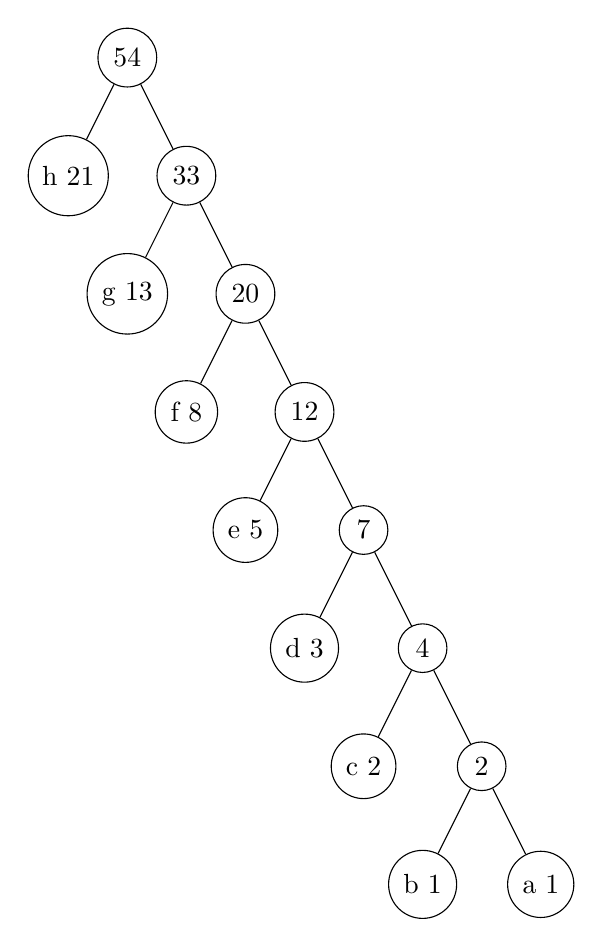
\begin{tikzpicture} \tikzstyle{every node}=[circle,draw]
\node {54}
    child {node {h 21}}
    child {node {33}
        child {node {g 13}}
        child {node {20}
            child {node {f 8}}
            child {node {12}
                child {node {e 5}}
                child {node {7}
                    child {node {d 3}}
                    child {node {4}
                        child {node {c 2}}
                        child {node {2}
                            child {node {b 1}}
                            child {node {a 1}}
                            }
                        }
                    }
                }
        }
    } ;
\end{tikzpicture}
\end{tabularx}

% 11. (b)
\item If $x$ is a node with only one child $y$ then $x$'s code is a prefix of $y$'s code. So the tree doesn't represent a prefix code.

% 11. (c)
\item

% 11. (d)
\item
%Proof by contradiction : suppose that $T'$ isn't optimal for $C'$. Let $T''$ be an optimal tree for $C'$. Let $\tilde{T}$ be the tree $T''$ with $x$ and $y$ as the children of $z$. $|\tilde{T}| < |T|$ wich contradicts the optimality of $T$.\\
%This proves the optimality of $T'$.\\
%Lets finally prove the optimality of Huffman's code. We will prove this result by induction on the size of the alphabet $C$.\\
%\begin{itemize}
%\item If $|C|=1$, Huffman codes are cleary optimal.
%\item If $|C| = n + 1$. Let $x$ and $y$ be the
%\end{itemize}

%Note that (c) and (d) prove the optimalitty of Huffman codes.

% 11. (e)
\item

\end{enumerate}
\end{enumerate}

\end{document}

